\subsubsection{$\phi \to \eta \gamma$ Decay}\label{sec:phi.etag}
The $\phi \rightarrow \eta \gamma $ decay is analogous to the $\etaP \rightarrow \gamma \gamma$ decay by replacing the initial pseudoscalar meson $P_p$with a vector meson $V_p$ and one of the $\gamma$ propagators with $\eta$. In this substitution 
\begin{align}\label{eq:phi.etag.amp}
{\cal M}(V_P(\epsilon_1) \to \eta(p) \gamma(\epsilon_2,k)) = {M}_V(p^2=m_{\eta},k^2=0) \varepsilon_{\mu\nu\rho\sigma}\epsilon_1^\mu p^\nu \epsilon_2^\rho k^\sigma
\end{align}
again, $\varepsilon_{\mu\nu\rho\sigma}$ is the antisymmetric metric tensor and the form factor, ${M}_V(p^2=\eta,k^2=0)$, contains information of the $\phi-\eta$ transition.

\subsubsection{\emph{Decay rate}}
The algebra for solving the squared matrix element is similar to Sec.~\ref{subsec:etaPMartix}, however since now the initial meson has polarization, a factor of 1/3~\cite{Hanhart2015} is introduced. The decay rate is also similar within a factor of 1/3 and can be represented as:
\begin{align}\label{eq:phi.etag.decay.final}
\Gamma_{V\rightarrow\eta\gamma} = \frac{1}{3} \frac{1}{64\pi} \left|M_{V}\right|^{2}\left(\frac{m_{\phi} - m_{\eta}}{m_{\phi}} \right)^{3} \ .
\end{align}
%\subsubsection{\emph{Decay rate}}
%The decay rate of a two-body decay is explained in Equation 46.17 of~\cite{pdg2014} as
%\begin{align}
%d\Gamma = \frac{1}{32 \pi^2} A \left|{\cal M}\right|^2\frac{\left|\bf{p_1}\right|}{m_p^2}d\Omega \ ,
%\end{align}
%where $d\Omega$ is the solid angle of particle 1 and $A$ is the symmetry factor which appears because of the Bose symmetry of the two
%outgoing photons. Substituting the square matrix element from Eq.~\ref{eq:piz_gg_amp_final} into Eq.~\ref{eq:pdg.2body} and integrating over the solid angle yields;
%\begin{align}
%\Gamma_{P\rightarrow\gamma\gamma} = \frac{1}{32\pi^{2}} \frac{1}{2} \left|{\cal M}(P_{P}\to\gamma(p)\gamma(k))\right|^{2} \frac{\left|\bf{p}\right|}{m_{P}^2} 4 \pi = \frac{1}{32 \pi}\left|M_{P}\right|^{2}m_{P}^{2}\left|\bf{p}\right|
%\end{align} 
%Finally, in the center-of-mass (C.M.) frame of the decaying meson, $\bf{p} = E_{\gamma}^{C.M.} = \frac{m_p}{2}$, we find the final expression of the decay rate of $P_P \to \gamma(\epsilon_1,p) \gamma(\epsilon_2,k)$ as;
%\begin{align}\label{eq:phi.etag.decay.final}
%\Gamma_{P\rightarrow\gamma\gamma} = \frac{1}{64\pi} \left|M_{P}\right|^{2}m_{P}^{3} \ .
%\end{align}


%
%\subsubsection{\emph{Photon Conversion to \epem Pairs}}\label{sec:intro.conversion}
%When a photon travels through matter at energies greater than 100~MeV, it can convert into an electron-positron pair. The process of pair production, $\gamma Z \rightarrow Ze^{+}e^{-}$, occurs when a photon with $E_0 > 2 m_e c^2$ converts into an electron and a positron. The cross section for this process can be written as;
%\begin{equation}\label{pair_crosssection}
%\sigma_{\gamma\rightarrow e^+e^-} =  \frac{A}{N_{A} \rho \lambda_\gamma}  \ ,\ \lambda_\gamma = \frac{9}{7}X_0
%\end{equation}
%where $\lambda$ is the interaction length, or mean free path, $\rho$ is the density of the material, $N_A$ is Avogadro's number and $A$ is the atomic mass of the material. The probability of pair production to occur is solely based on $X_{0}$, the radiation length of the medium and this probability can be expressed as;
%\begin{equation}
%\frac{dP}{dx} = \frac{1}{\lambda_\gamma}\exp(\frac{-x}{\lambda_\gamma}) \ .
%\end{equation}
%%
%%
%The probability of pair production when a photon, from the $\etaP \to \gamma \gamma$ decay, traveling though 5~cm of liquid hydrogen, $\ell$H$_2$, is shown in Fig.~\ref{fig:conversion} as well as the number of $\etaP \to \gamma \gamma \rightarrow e^+e^- \gamma$ / $100 \etaP \rightarrow e^+e^- \gamma$. 
%\begin{figure}[h!]\begin{center}
%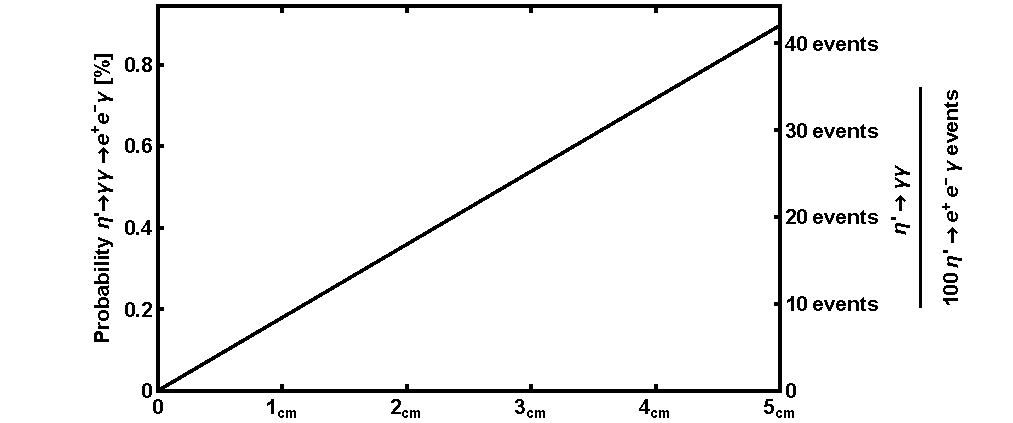
\includegraphics[width=\figwidth,height=\qfigheight]{\grpath/decays/cmplot.pdf}
%\caption[Probability of pair production, $\gamma \to$\epem, as a function of distance in liquid hydrogen]{\label{fig:conversion}{(Left axis)Probability of pair production, $\gamma \to$\epem; (Right axis) number of $\etaP \to \gamma \gamma \rightarrow e^+e^- \gamma$ / $100 \etaP \rightarrow e^+e^- \gamma$ as a function of distance in liquid hydrogen.}}
%\end{center}\end{figure}
%Since CLAS12 has a vertex resolution of $\approx$1~mm the probability of pair production traveling through 10~mm is shown in Fig.~\ref{fig:conversionmm}. Therefore, a 1~mm cut on the primary vertex will yield a contamination of $\approx$ one externally converted \epem from $\etaP \to \gamma \gamma \rightarrow e^+e^- \gamma$ per Dalitz decays $100 \etaP \rightarrow e^+e^- \gamma$
%\begin{figure}[h!]\begin{center}
%		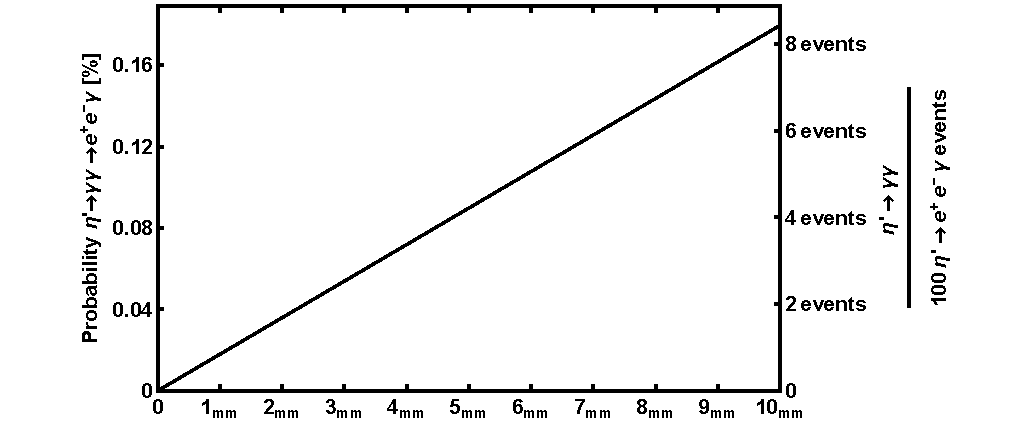
\includegraphics[width=\figwidth,height=\qfigheight]{\grpath/decays/mmplot.pdf}
%		\caption[Probability of pair production, $\gamma \to$\epem, as a function of distance in liquid hydrogen]{\label{fig:conversionmm}{(Left axis)Probability of pair production, $\gamma \to$\epem; (Right axis) number of $\etaP \to \gamma \gamma \rightarrow e^+e^- \gamma$ / $100 \etaP \rightarrow e^+e^- \gamma$ as a function of distance in liquid hydrogen.}}
%	\end{center}\end{figure}
%This type of subprocess mimics the Dalitz decay  $\etaP \to e^+e^- \gamma$, described in Sec.~\ref{sec:dalitzdecay}. Since there are two photons with equal probability of conversion, the total probabilities shown is for when either photon externally converts.
%

